\documentclass[10pt,a4paper]{article}
\usepackage[margin=1.5cm,top=1.25cm,bottom=1.3cm]{geometry}
\usepackage{amsmath,amssymb}
\usepackage{graphicx}
\usepackage{booktabs}
\usepackage{xcolor}
\usepackage[hidelinks]{hyperref}
\usepackage{caption}
\usepackage{titlesec}
\captionsetup{font=footnotesize,labelfont=bf,skip=2pt}
\titleformat{\section}{\normalfont\bfseries}{\thesection}{0.6em}{}
\titlespacing*{\section}{0pt}{5pt}{1pt}
\setlength{\parskip}{1.5pt plus 1pt}
\setlength{\parindent}{0pt}
\setlength{\abovedisplayskip}{3pt}\setlength{\belowdisplayskip}{3pt}
\setlength{\textfloatsep}{6pt plus 2pt}
\newcommand{\code}[1]{\texttt{#1}}
\newcommand{\PH}[1]{\textcolor{red}{[#1]}}
\begin{document}
{\centering
{\large\bfseries Support-aware training of hard Top-$K$ under the code residual without a surrogate backward}\\[1pt]
{\small 8-layer TinyStories models of the K+J notes, \code{code\_residual}, abs-TopK over \(N=1536\); runs \code{ma\_alt\_*} (madrid), configs \code{configs/cr\_kj/alt/}.}\par}

\section{Question}
The K+J notes ask for a hard Top-\(K\) model whose training is aware of other supports: candidates just outside
the support should receive a signal about whether they belong in it.  RBLapSum supplies that signal as a surrogate
backward -- a relaxed Jacobian \(M+S\) of the gate, with \(S\) the kernel-weighted exchange term over the
Top-\((K{+}J)\) pool -- and under the code residual, where the gate's output is also a skip connection, the relaxed
Jacobians of successive gates multiply along the carry (\code{docs/carry-surrogate.tex}).  Fixing that by
re-routing gradients is a repair of a surrogate that does not fit the architecture.  This note asks the question
the other way round: which training rules give the candidates a signal \emph{without} a surrogate backward, so
that nothing can compound because every backward is the exact gradient of some forward?

\section{Three candidates}
\textbf{A. Stochastic support width} (\code{stochastic\_width}).  Every forward is a hard Top-\(K'\) forward; per
token, \(K'\) is drawn from a distribution on \(\{K,\dots,K{+}J\}\) in training and is \(K\) at evaluation.  The
objective is \(\mathbb E_{K'}\,\mathcal L(K')\) and the gradient is exact; a candidate at rank \(K{+}m\) is active,
and trained, with probability \(P(K'\ge K{+}m)\), so the distribution on \(K'\) \emph{is} the probability
distribution on the pool, realized in the forward instead of in the backward.  Three distributions: uniform on
\([K,K{+}J]\); two-point (\(K{+}J\) with probability \(\tfrac12\), else \(K\)); geometric excess with mean \(J/4\).
This is the width sampling of universally slimmable networks (Yu \& Huang 2019) and the nested training of
Matryoshka SAEs (Bussmann et al.\ 2025) applied to the support, with the smallest width as the deployed one.
Under the code residual the carried code is hard at every width, so the carry is exact by construction.

\textbf{B. Soft straight-through} (\code{surrogate\_mode=soft\_ste}).  Hard forward; backward Jacobian
\(M+(1-M)\,p\) over the pool, \(p_i=F((|u_i|-b)/T)\) the kernel's CDF: a candidate receives the gradient it would
receive if present, weighted by its probability of being present.  No exchange term.  Every per-coordinate gain
is at most one, so the products along the carry are bounded by one; the price is that the candidates' values are
trained on a counterfactual, as in any straight-through estimator (Bengio et al.\ 2013; JumpReLU SAEs,
Rajamanoharan et al.\ 2024).

\textbf{C. RBLapSum on the candidates only} (\code{rblapsum\_surrogate\_scope=inactive}).  The support term is
applied to the \(J\) inactive members and the \(K\) active ones keep the exact gradient.  The argument: the active
values already have a gradient, and if the loss wants one smaller it shrinks and leaves; only the entry decision is
blind.  A candidate is not carried (its code value is zero), so the term is applied once per entry event and
cannot compound along the identity.

\section{Results}

\textbf{Setup.}  The code-carried cells of the K+J grid, 3000-step screens with the grid's 20k schedule untouched,
eight RTX 5090 (the grid's own machine), step-matched against the grid's hard Top-\(K\) baselines (post-norm) and
its RBLapSum \code{pool} cells; the carry-scope results of \code{docs/carry-surrogate.tex} are shown for reference.
Candidate A trains the hard baseline's own config (post-norm) with a random width; B and C train the \code{pool}
cell's config (no post-norm, \(T=2\)) with one field changed.

\begin{figure}[b]
\centering
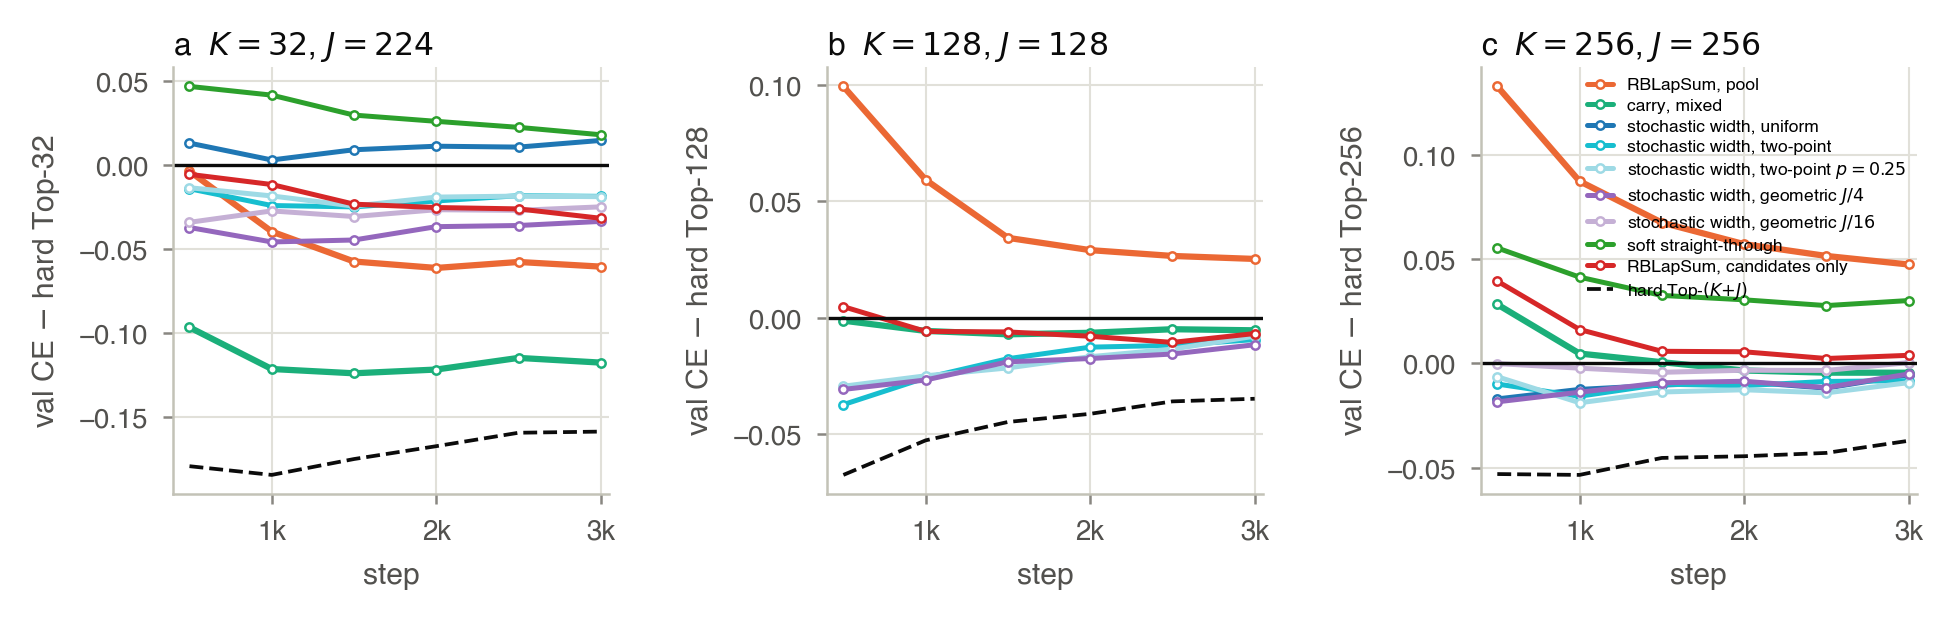
\includegraphics[width=\textwidth]{figures/carry/fig_alt.png}
\caption{Validation CE minus the code-carried hard Top-\(K\) baseline over the first 3000 steps; dashed, hard
Top-\((K{+}J)\).  \textbf{a} \((32,224)\); \textbf{b} \((128,128)\); \textbf{c} \((256,256)\).}
\label{fig:alt}
\end{figure}

\textbf{At step 3000, minus hard Top-\(K\)} (Fig.~\ref{fig:alt}, Table~\ref{tab:alt}).  At \((256,256)\), the cell
where the unmodified surrogate loses \(0.047\), every width distribution except the narrowest beats the hard model
-- two-point \(-0.008\) and \(-0.009\) (\(p=\tfrac12\), \(\tfrac14\)), uniform \(-0.006\), geometric \(J/4\) \(-0.005\),
geometric \(J/16\) \(0.000\) -- with no surrogate and no gradient modification, as much as the best carry scope
(\(-0.005\)); candidates-only RBLapSum ends at \(+0.004\), the soft straight-through at \(+0.030\).  At \((128,128)\)
the widths give \(-0.012\) (geometric \(J/4\)), \(-0.010\) (two-point) and \(-0.008\) (two-point \(p=\tfrac14\)),
against \(-0.006\) for the mixed carry scope and \(-0.007\) for candidates-only RBLapSum (\code{pool} \(+0.025\)).  At \((32,224)\) the order of the width
distributions follows how much mass they put near \(K\): uniform \(+0.014\), two-point \(-0.019\) at both \(p=\tfrac12\)
and \(\tfrac14\), geometric \(J/16\) \(-0.025\), geometric \(J/4\) \(-0.034\); at \((64,64)\) the two-point and geometric widths give
\(-0.029\) and \(-0.023\) (\code{pool} \(-0.005\), mixed carry scope \(-0.047\), hard Top-128 \(-0.059\)); candidates-only RBLapSum \(-0.032\), soft
straight-through \(+0.018\), the unmodified surrogate \(-0.061\), the mixed carry scope \(-0.118\).
\PH{10k continuations}

\begin{figure}[t]
\centering
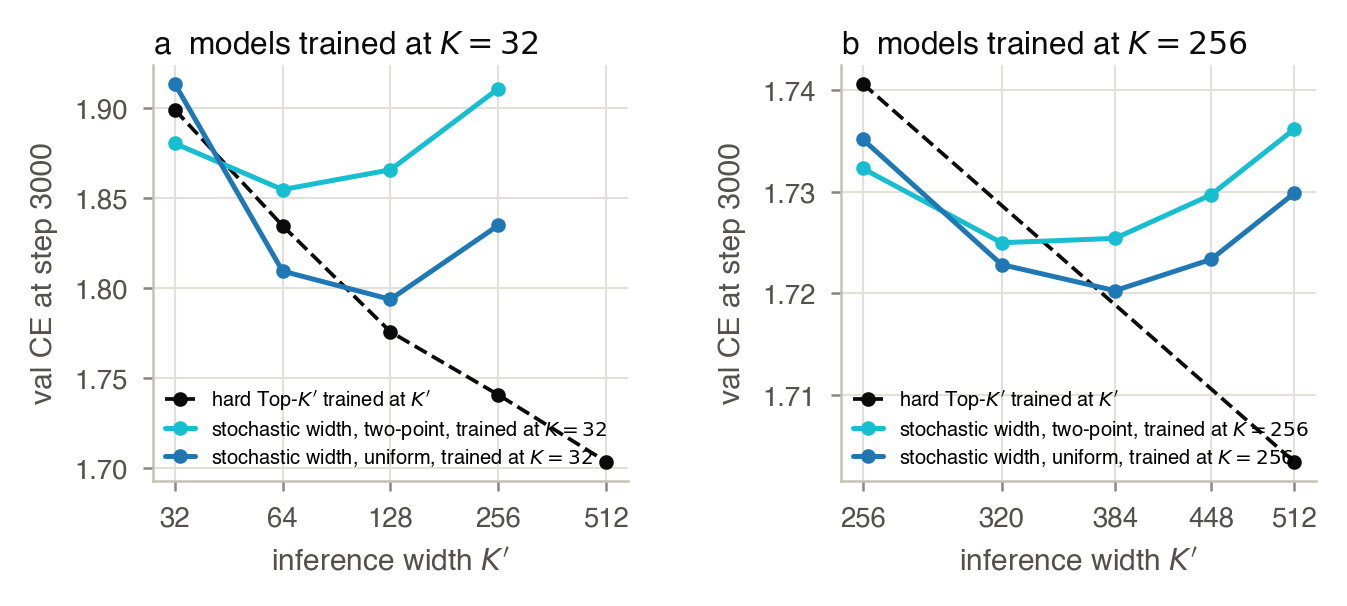
\includegraphics[width=.74\textwidth]{figures/carry/fig_widths.png}
\caption{One checkpoint, several inference widths: validation CE at step 3000 of the stochastic-width models
evaluated with hard Top-\(K'\) for \(K'\) in their training range, against the grid's hard models trained at each
\(K'\) (\code{analysis/eval\_widths.py}).}
\label{fig:widths}
\end{figure}

\textbf{What a stochastic-width model is} (Fig.~\ref{fig:widths}).  Evaluated across its training range, the model
is not a slimmable ladder: its loss is lowest at an intermediate width and rises again toward \(K{+}J\), where it is
far above the hard model trained there (\(1.736\) against \(1.703\) at \(K'=512\)).  At the narrow end it beats the hard
models: the uniform model trained at \(K=32\) gives \(1.809\) at \(K'=64\) against \(1.835\) for hard Top-64, and both
\(K=256\) models beat hard Top-256 at \(K'=256\).  The random width acts as a regularizer on the support -- the
network cannot rely on any particular candidate being present -- rather than as a way of training several models
at once.

\begin{table}[t]
\centering\footnotesize
\begin{tabular}{llcccccccc}
\toprule
 & & & & \multicolumn{4}{c}{stochastic width} & & \\
\cmidrule(lr){5-8}
\(K\) & \(J\) & pool & carry mixed & uniform & two-point & geom.\ \(J/4\) & geom.\ \(J/16\) & soft STE & cand.\ only \\
\midrule
32 & 224 & \(-0.061\) & \(\mathbf{-0.118}\) & \(+0.014\) & \(-0.019\) & \(-0.034\) & \(-0.025\) & \(+0.018\) & \(-0.032\) \\
64 & 64 & \(-0.005\) & \(\mathbf{-0.047}\) & -- & \(-0.029\) & \(-0.023\) & -- & -- & -- \\
128 & 128 & \(+0.025\) & \(-0.006\) & -- & \(-0.010\) & \(\mathbf{-0.012}\) & -- & -- & \(-0.007\) \\
256 & 256 & \(+0.047\) & \(-0.005\) & \(-0.006\) & \(\mathbf{-0.008}\) & \(-0.005\) & \(0.000\) & \(+0.030\) & \(+0.004\) \\
\bottomrule
\end{tabular}
\caption{Validation CE at step 3000 minus the code-carried hard Top-\(K\) of the row (\(1.899\), \(1.835\), \(1.776\), \(1.741\)); two-point with \(p=\tfrac12\). Bold: best of the row.}
\label{tab:alt}
\end{table}

\section{Reading}

\textbf{The probability distribution on the pool can live in the forward.}  RBLapSum puts a distribution on the
Top-\((K{+}J)\) pool and differentiates through it; under the carry that derivative compounds because the same
carried value is relaxed at every gate.  Sampling the width puts the distribution on the pool into the forward
instead -- a candidate at rank \(K{+}m\) is present with probability \(P(K'\ge K{+}m)\) and, when present, is trained
by the exact gradient of a hard forward -- so there is no surrogate Jacobian, nothing to route, and the carried code
is a hard code at every step.  At \((256,256)\) this is enough: every width distribution tried beats the hard model
(\(-0.005\) to \(-0.008\)), the carry scopes' result without the carry scopes.  The price is a train/test mismatch
on the support width: the deployed model has seen its own width only part of the time, and the gap to the hard
baseline at \(K=32\) depends on how much of the distribution sits at \(K\) (uniform \(+0.014\), two-point
\(-0.019\), geometric \(J/16\) \(-0.025\), geometric \(J/4\) \(-0.034\)).  Where the unmodified surrogate is worth
\(0.06\) and the mixed carry scope \(0.12\), the best width distribution tried is worth \(0.034\).

\textbf{What the hard forward cannot give the candidates.}  The two surrogate-free rules differ in what a
candidate learns from.  Under the stochastic width it learns from being \emph{present}, in a forward where the
whole stack adapts to its presence; under the soft straight-through it learns from a counterfactual, the gradient
it would receive if present, with the rest of the stack unchanged.  The second is worse than the hard backward at
both \(K\) (\(+0.018\), \(+0.030\)), while RBLapSum restricted to the same candidates with its boundary exchange
term (\(-0.032\), \(+0.004\)) is not: the value of RBLapSum's signal is the \emph{relative} ranking of candidates
near the boundary, not the counterfactual gradient as such.

\textbf{Against the carry scopes.}  The carry scopes keep RBLapSum's signal, including the eviction term that the
measurements of \code{docs/carry-surrogate.tex} found decisive at \(K=32\), and make it compatible with the carry
by a rule about where the kernel acts.  The stochastic width is the natural surrogate-free training of a hard
Top-\(K\) under the code residual and matches them at large \(K\), where the hard model's own selection is already
good and the surrogate's job is only to keep candidates alive; at small \(K\), where the selection itself is
worth \(0.1\) nats, a distribution over widths does not reach what a gradient on the ranking does.  \PH{10k}

\textbf{Scope.}  One seed, 3000-step screens (one 10k continuation), the \(T=2\) code-carried family of the K+J
grid; the stochastic-width models carry the post-norm of the hard baselines, the surrogate cells do not (worth
about \(0.007\) to a hard model in the stream grid).

\end{document}
